\PassOptionsToPackage{activate={false}}{microtype}
\documentclass[alpha-refs]{wiley-article}

\usepackage{graphicx}
\usepackage[space]{grffile}
\usepackage{latexsym}
\usepackage{textcomp}
\usepackage{longtable}
\usepackage{tabulary}
\usepackage{booktabs,array,multirow}
\usepackage{amsfonts,amsmath,amssymb}
\usepackage{natbib}
\usepackage{url}
\usepackage{placeins}
\usepackage{hyperref}
\hypersetup{colorlinks=false,pdfborder={0 0 0}}
\usepackage[utf8]{inputenc}
\usepackage[english]{babel}
\usepackage{siunitx}
\usepackage{algorithm}
\usepackage{algpseudocode}

\newif\iflatexml\latexmlfalse
\providecommand{\tightlist}{\setlength{\itemsep}{0pt}\setlength{\parskip}{0pt}}

\iflatexml
\else
\paperfield{Systems Engineering Journal}
\fi

\papertype{Supplementary Material}

\title{Supplementary Material: Understanding Software Engineering Organizations Through Systems Thinking}

\author[1]{Juliana Alves}
\author[1,2]{Henrique Alves}
\author[1,3]{André Costa Batista}

\affil[1]{Systems Engineer, Steiner Institute, Cherenkov Telescope Array Observatory (CTAO) - São Paulo, SP, Brazil}
\affil[2]{Graduate Program in Electrical Engineering - Universidade Federal de Minas Gerais - Av. Antônio Carlos 6627, 31270-901, Belo Horizonte, MG, Brazil}
\affil[3]{Department of Electrical Engineering - Universidade Federal de Minas Gerais - Av. Antônio Carlos 6627, 31270-901, Belo Horizonte, MG, Brazil}

\runningauthor{Alves, Alves, and Batista}

\begin{document}

\maketitle

\section*{Nomenclature}

\subsection*{State Variables}
\begin{tabular}{ll}
$F$ & Product feature completeness \\
$D$ & Technical debt accumulation \\
$B$ & Bug count \\
$M$ & Market share (\%) \\
$F_m$ & Product-market fit \\
$A_{brand}$ & Brand awareness \\
$A_{org}$ & Organizational alignment \\
$C_{org}$ & Organizational conflict \\
$Q_{prod}$ & Product quality (composite metric) \\
$R$ & Financial runway (months) \\
$C_{i,j}$ & Capacity $j$ of agent $i$ \\
$V_{agg}$ & Aggregate development velocity \\
$S_{cap}$ & Sales capacity \\
$L_{context}$ & Learning context factor \\
$S_{stress}$ & Stress factor
\end{tabular}

\subsection*{Parameters - Flow Rates}
\begin{tabular}{ll}
$\lambda_{feat}$ & Feature development rate coefficient \\
$\lambda_{debt}$ & Technical debt generation rate \\
$\lambda_{bugs}$ & Bug introduction rate \\
$\lambda_{acq}$ & Customer acquisition rate coefficient \\
$\mu_F$ & Feature deprecation rate \\
$\rho_{refactor}$ & Refactoring effectiveness coefficient \\
$\rho_{fix}$ & Bug fixing effectiveness coefficient
\end{tabular}

\subsection*{Parameters - Drag and Quality}
\begin{tabular}{ll}
$\delta_{debt}$ & Technical debt drag coefficient \\
$\alpha_{qual}$ & Quality investment allocation parameter \\
$\alpha_{HR}$ & Human Resources coordination capacity (normalized) \\
$\kappa$ & Code quality factor \\
$\tau$ & Quality consciousness parameter
\end{tabular}

\subsection*{Parameters - Financial}
\begin{tabular}{ll}
$\gamma_{rev}$ & Revenue conversion coefficient \\
$\beta_{burn}$ & Per-employee monthly burn rate \\
$\beta_{overhead}$ & Fixed operational overhead \\
$F_{funding}(t)$ & Funding events at time $t$
\end{tabular}

\subsection*{Parameters - Organizational Dynamics}
\begin{tabular}{ll}
$\eta_{learn}$ & Base learning rate \\
$\eta_{decay}$ & Capability degradation rate \\
$\tau_{base}$ & Baseline monthly turnover probability \\
$\xi_{decay}$ & Organizational alignment decay rate \\
$\xi_{conflict}$ & Conflict impact coefficient \\
$\chi_{base}$ & Baseline customer churn rate \\
$\chi_{bugs}$ & Bug-driven churn coefficient \\
$\chi_{misfit}$ & Market misfit churn coefficient
\end{tabular}

\subsection*{Other Notation}
\begin{tabular}{ll}
$n_{total}$ & Total organizational headcount \\
$i$ & Agent index \\
$j$ & Capacity type index \\
$k$ & Management agent index \\
$h$ & Human Resources agent index \\
$t$ & Time (months)
\end{tabular}

\section{Simulation Algorithm}
\label{app:algorithm}

Algorithm~\ref{alg:simulation} formalizes the core simulation loop executed each monthly timestep. The algorithm integrates agent capacity evolution, role-specific actions, state updates, strategic decisions, financial dynamics, and team turnover within a unified framework that ensures proper causal ordering.

\begin{algorithm}[!htbp]
\caption{Monthly Organizational Simulation Step}
\label{alg:simulation}
\begin{algorithmic}[1]
\State \textbf{Input:} State $S_t$, Agents $\mathcal{A}$, Parameters $\Theta$
\State \textbf{Output:} State $S_{t+1}$

\For{each agent $a \in \mathcal{A}$}
    \State Update capacities: $\Delta C_a \leftarrow \eta_{learn} L_{context}(100-C_a) - \eta_{decay} S_{stress} C_a$
\EndFor

\State Compute aggregate outputs by role:
\State \quad Engineers: $\Delta F, \Delta D, \Delta B$ from development velocity $V_{agg}$ with debt drag
\State \quad Sales: $\Delta M_{acq}$ from sales capacity, product quality, brand, market saturation
\State \quad Marketing: $\Delta A_{brand}$, lead quality from marketing capacity
\State \quad HR: $\Delta A_{org,HR}$, conflict resolution from coordination capacity
\State \quad Management: $\Delta A_{org,mgmt}$ from management capacity

\State Update product \& organizational state: $F, D, B, M, A_{brand}, A_{org}, C_{org}$

\If{crisis detected (debt, bugs, or market misfit)}
    \State Adjust strategy: increase $\alpha_{quality}$ or reallocate effort
\EndIf

\If{pivot conditions met}
    \State Execute pivot (reset product, retain team)
\EndIf

\State Compute finances: $Revenue \leftarrow \gamma_{rev} M Q_{prod}$; $Burn \leftarrow \beta_{burn}|\mathcal{A}| + \beta_{overhead}$
\State Update runway: $R \leftarrow R + Revenue - Burn + F_{funding}(R, Q_{prod}, M)$

\For{each agent $a$}
    \If{random() $< P_{turnover}(HR_{eff}, C_{org})$}
        \State Replace $a$ with new agent
    \EndIf
\EndFor

\If{$R \leq 0$} \Return \textsc{Failure}
\ElsIf{$t > t_{max}$} \Return \textsc{Success}
\EndIf

\State \Return $S_{t+1}$
\end{algorithmic}
\end{algorithm}

The algorithm implements seven phases: (1) agent capacity evolution through learning and degradation; (2) role-specific actions producing technical, market, and organizational changes; (3) state integration with feedback dynamics; (4) strategic interventions based on crisis thresholds; (5) financial computation with revenue, burn, and funding; (6) probabilistic turnover and hiring; (7) termination evaluation.

\section{State Evolution Equations}
\label{app:equations}

This appendix presents the formal mathematical specifications for state variable evolution. All equations are implemented in discrete-time simulation with monthly timesteps.

\subsection{Technical Subsystem Dynamics}

\textbf{Feature Completeness:}
\begin{equation}
\frac{dF}{dt} = \lambda_{feat} \sum_i C_{dev,i} \cdot (1 - \delta_{debt}(D)) - \mu_F \cdot F
\end{equation}
where the debt drag function implements saturation dynamics:
\begin{equation}
\delta_{debt}(D) = \frac{D}{D + 200}
\end{equation}
and $\mu_F \approx 0$ (feature deprecation negligible).

\textbf{Quality Focus Factor:}
Engineering teams exhibit heterogeneous quality consciousness. To prevent the pathological case where $\overline{C_{exp}} \approx \overline{C_{dev}}$ (leading to $\tau \approx 1$ and $(1-\tau) \approx 0$, which artificially eliminates debt/bug generation), we normalize quality focus as:
\begin{equation}
\tau = \min\left(\frac{\overline{C_{exp}}}{100}, 0.8\right)
\end{equation}
This ensures $(1-\tau) \in [0.2, 1.0]$, creating debt accumulation dynamics even when teams have high explanation capacity.

\textbf{Technical Debt Evolution:}
\begin{equation}
\frac{dD}{dt} = \lambda_{debt} \cdot V_{agg} \cdot (1 - \tau) - \rho_{refactor} \cdot W_{refactor}
\end{equation}
where $V_{agg}$ is aggregate development velocity, $W_{refactor}$ is refactoring work allocation, and $\rho_{refactor} = 0.04$ represents refactoring effectiveness.

\textbf{Exponential Velocity Penalty:}
Technical debt imposes a non-linear drag on development velocity:
\begin{equation}
\delta_{debt}(D) = \frac{1}{1 + (D/50)^2}
\end{equation}
This exponential penalty ensures that accumulated debt ($D > 100$) drastically reduces productivity, creating the feedback dynamics of Loop R1. When $D > 200$, the system enters technical bankruptcy (game over condition).

\textbf{Code Quality Evolution:}
\begin{equation}
\frac{dQ_c}{dt} = \gamma_{refactor} \cdot W_{refactor} - \gamma_{decay} \cdot D
\end{equation}
with $\gamma_{refactor} = 0.01$ and $\gamma_{decay} = 0.01$, implementing bidirectional coupling between quality and debt.

\textbf{Bug Count Evolution:}
\begin{equation}
\frac{dB}{dt} = \lambda_{bugs} \cdot V_{agg} \cdot \kappa(Q_c) \cdot (1 - \tau) - \rho_{fix} \cdot W_{bugfix}
\end{equation}
where the quality modulation function is:
\begin{equation}
\kappa(Q_c) = \frac{100 - Q_c}{100}
\end{equation}
and $\rho_{fix}$ represents bug fixing efficiency.

\textbf{Bug Velocity Penalty:}
Bugs impose exponential drag on development velocity:
\begin{equation}
\delta_{bugs}(B) = \frac{1}{1 + (B/20)^{1.5}}
\end{equation}
Beyond critical thresholds ($B > 100$), the system becomes unmaintainable, triggering game over.

\subsection{Resource Allocation Strategy}

Engineering capacity is allocated according to strategic parameters $\alpha_{dev}$ and $\alpha_{features}$:
\begin{align}
W_{dev} &= C_{available} \cdot \alpha_{dev} \\
W_{quality} &= C_{available} \cdot (1 - \alpha_{dev}) \\
W_{features} &= W_{dev} \cdot \alpha_{features} \\
W_{refactor} &= W_{dev} \cdot (1 - \alpha_{features}) \\
W_{bugfix} &= W_{quality}
\end{align}
where $C_{available}$ is total available engineering capacity.

\subsection{Market Subsystem Dynamics}

\textbf{Product Quality Composite:}
\begin{equation}
Q_{prod} = \frac{F_m}{100} \cdot \frac{F}{F + 50} \cdot \left(1 - \frac{B}{B + 50}\right)
\end{equation}
combining market fit, feature completeness (with saturation), and bug-free operation.

\textbf{Lead Quality:}
\begin{equation}
L_q = \text{clip}\left(\frac{\overline{C_{pub}} + \overline{C_{ideas}}}{2} \cdot Q_{prod}, 0, 100\right)
\end{equation}
where $\overline{C_{pub}}$ and $\overline{C_{ideas}}$ are mean marketing capacities.

\textbf{Brand Awareness Growth:}
\begin{equation}
\frac{dA_{brand}}{dt} = \omega_{mkt} \cdot M_{eff} \cdot \left(1 - \frac{A_{brand}}{100}\right) - \mu_{brand} \cdot A_{brand}
\end{equation}
where $M_{eff}$ is effective marketing effort and decay $\mu_{brand}$ represents brand erosion.

\textbf{Market Share Dynamics:}
\begin{equation}
\frac{dM}{dt} = \lambda_{acq} \cdot S_{cap} \cdot Q_{prod} \cdot A_{brand} \cdot (1-M/100)^2 - \chi_{total} \cdot M
\end{equation}
where total churn is:
\begin{equation}
\chi_{total} = \chi_{base} + \chi_{bugs} \cdot \frac{B}{B + 50} + \chi_{misfit} \cdot \left(1 - \frac{F_m}{100}\right)
\end{equation}
implementing multi-factor attrition.

\subsection{Organizational Subsystem Dynamics}

\textbf{Organizational Alignment:}
\begin{equation}
\frac{dA_{org}}{dt} = \sum_k C_{mgmt,k} + \sum_h C_{coord,h} - \xi_{decay} \cdot A_{org} - \xi_{conflict} \cdot C_{org}
\end{equation}
with half-life approximately 15 months without active management ($\xi_{decay} \approx 0.047$).

\textbf{Conflict Generation:}
\begin{equation}
\frac{dC_{org}}{dt} = \gamma_{misalign} \cdot \left(1 - \frac{A_{org}}{100}\right) + \gamma_{pressure} \cdot \frac{B}{B + 50} - \rho_{HR} \cdot \sum_h C_{resolve,h}
\end{equation}
where $\gamma_{misalign} = 0.3$ and $\gamma_{pressure} = 0.2$ represent conflict generation rates, and $\rho_{HR}$ is HR resolution effectiveness.

\subsection{Financial Dynamics}

\textbf{Revenue Generation:}
\begin{equation}
R_{revenue} = \gamma_{rev} \cdot Q_{prod} \cdot S_{power} \cdot M
\end{equation}
where sales power is:
\begin{equation}
S_{power} = \overline{C_{sell}} \cdot n_{sales}
\end{equation}
with $\overline{C_{sell}}$ mean selling capacity and $n_{sales}$ sales team size.

\textbf{Cash Runway Evolution:}
\begin{equation}
\frac{dR_{cash}}{dt} = R_{revenue} + F_{funding}(t) - (\beta_{burn} \cdot n_{total} + \beta_{overhead})
\end{equation}
where runway depletion ($R_{cash} \leq 0$) triggers crisis protocols or venture termination.

\subsection{Quality Penalties on Revenue}

Product quality defects directly impact revenue generation through exponential penalty functions:
\begin{equation}
\text{bug\_penalty} = \frac{1}{1 + (B/30)^2}
\end{equation}
\begin{equation}
\text{debt\_penalty} = \frac{1}{1 + (D/80)^{1.5}}
\end{equation}
These penalties multiply with $R_{revenue}$, ensuring that technical shortcuts eventually erode market performance.

\subsection{Game Over Conditions}

The model implements three terminal conditions:
\begin{enumerate}
\item Financial Bankruptcy: $R_{cash} \leq 0$ (cash runway exhausted)
\item Technical Bankruptcy: $D > 200$ (technical debt exceeds maintainability threshold)
\item Quality Crisis: $B > 100$ (bug count exceeds customer tolerance)
\end{enumerate}
These conditions formalize the multi-dimensional failure modes observed in software ventures.

\subsection{Capacity Evolution Mechanisms}

Agent capabilities evolve through learning and degradation processes:
\begin{equation}
\Delta C_{i,j} = \eta_{learn} \cdot L_{context} \cdot (100 - C_{i,j}) - \eta_{decay} \cdot S_{stress} \cdot C_{i,j}
\end{equation}
where learning context incorporates:
\begin{equation}
L_{context} = L_{base} \cdot \left(1 + \frac{A_{org}}{100}\right) \cdot \left(1 + \frac{TD_{boost}}{100}\right) \cdot F_{focus}
\end{equation}
with $TD_{boost}$ representing HR talent development contribution and $F_{focus}$ strategic focus alignment.

Stress factors include:
\begin{equation}
S_{stress} = S_{base} \cdot \left(1 + \frac{C_{org}}{100}\right) \cdot \left(1 + \frac{B}{B + 50}\right)
\end{equation}
implementing degradation under conflict and quality crises.

\textbf{Turnover Dynamics:}
\begin{equation}
P_{turnover} = \tau_{base} \cdot \left(1.5 - \frac{\overline{C_{HR}}}{100}\right) \cdot \left(1 + 0.5 \cdot \frac{C_{org}}{100}\right)
\end{equation}
where $\tau_{base} = 0.02$ (2\% monthly baseline) and $\overline{C_{HR}}$ represents normalized HR coordination capacity.

\section{State Variable Specifications}
\label{app:stockflow}

This section provides detailed mathematical specifications for each of the six primary state variables and their governing equations.

\subsection{Product Features ($F$)}

Accumulated functionality representing product scope. Growth is non-linear due to technical debt's velocity penalty ($\delta_{debt} \cdot D$), creating path-dependent development trajectories where early shortcuts compound into long-term velocity loss.

\textbf{Equation:}
\begin{equation}
\frac{dF}{dt} = \lambda_{feat} \sum_i C_{dev,i} \cdot (1 - \delta_{debt} \cdot D) - \mu_F \cdot F
\end{equation}

\noindent where $\mu_F \approx 0$ (negligible deprecation), $\lambda_{feat}$ is the feature development rate coefficient, $C_{dev,i}$ is development capacity of engineer $i$, and $\delta_{debt}$ is the technical debt drag coefficient.

\subsection{Technical Debt ($D$)}

Accumulated design compromises and shortcuts. Represents debt principal ($D$), while the debt drag coefficient ($\delta_{debt}$) operationalizes interest as an ongoing productivity tax on feature development.

\textbf{Equation:}
\begin{equation}
\frac{dD}{dt} = \lambda_{debt} \cdot V_{agg} \cdot (1 - \tau) - \rho_{refactor} \cdot W_{refactor}
\end{equation}

\noindent with exponential penalty $\delta_{debt}(D) = 1/(1+(D/50)^2)$, implementing Loops R1/B1. Here $\lambda_{debt}$ is the technical debt generation rate, $V_{agg}$ is aggregate development velocity, $\tau$ is quality consciousness parameter, $\rho_{refactor}$ is refactoring effectiveness coefficient, and $W_{refactor}$ is refactoring work allocation.

\subsection{Bug Count ($B$)}

Known defects awaiting resolution. Exhibits threshold behavior---beyond critical levels ($B > 30$), bugs cascade through system interdependencies faster than resolution capacity, triggering Loop R2 (Bug Accumulation) if not arrested by crisis management.

\textbf{Equation:}
\begin{equation}
\frac{dB}{dt} = \lambda_{bugs} \cdot V_{agg} \cdot \kappa \cdot (1-\tau) - \rho_{fix} \cdot W_{bugfix}
\end{equation}

\noindent with penalty $\delta_{bugs}(B) = 1/(1+(B/20)^{1.5})$, implementing Loop R2. Here $\lambda_{bugs}$ is the bug introduction rate, $\kappa$ is code quality factor, $\rho_{fix}$ is bug fixing effectiveness coefficient, and $W_{bugfix}$ is bug fixing work allocation.

\subsection{Market Share ($M$)}

Captured market percentage ($M \in [0,100]$). Saturation effects create diminishing returns: $(1 - M)^2$ models increasing difficulty of capturing remaining market. Multi-factor churn (base, bug-driven, misfit-driven) implements Loop B2 (Market Feedback).
\textbf{Equation:}
\begin{equation}
\frac{dM}{dt} = \lambda_{acq} S_{cap} Q_{prod} A_{brand} (1-M)^2 - (\chi_{base} + \chi_{bugs} B + \chi_{misfit}(100-F_m))M
\end{equation}

\noindent where $\lambda_{acq}$ is customer acquisition rate coefficient, $S_{cap}$ is sales capacity, $Q_{prod}$ is product quality, $A_{brand}$ is brand awareness, $\chi_{base}$ is baseline customer churn rate, $\chi_{bugs}$ is bug-driven churn coefficient, $\chi_{misfit}$ is market misfit churn coefficient, and $F_m$ is product-market fit. The saturation constraint $(1-M)^2$ implements Loops R3/B2.

\subsection{Organizational Alignment ($A_{org}$)}

Degree of strategic coherence across teams ($A_{org} \in [0,100]$). Acts as a capacity multiplier---misaligned organizations waste effort on internal friction rather than value creation. Natural entropy ($\xi_{decay}$) requires continuous management and HR coordination to sustain, implementing Loop B4 dynamics.

\textbf{Equation:}
\begin{equation}
\frac{dA_{org}}{dt} = \sum_k C_{mgmt,k} + \sum_h C_{coord,h} - (\xi_{decay} A_{org} + \xi_{conflict} C_{org})
\end{equation}

\noindent where $C_{mgmt,k}$ is management capacity of manager $k$, $C_{coord,h}$ is coordination capacity of HR agent $h$, $\xi_{decay}$ is organizational alignment decay rate (half-life $\approx$ 15 months without active management), $\xi_{conflict}$ is conflict impact coefficient, and $C_{org}$ is organizational conflict level.

\subsection{Financial Runway ($R$)}

Available capital measured in months of operation ($R$). Revenue inflow depends on market share and product quality; burn rate scales linearly with headcount plus fixed overhead. Depletion triggers crisis responses (layoffs, pivots) or venture failure, implementing critical constraint on organizational dynamics.

\textbf{Equation:}
\begin{equation}
\frac{dR}{dt} = \gamma_{rev} M Q_{prod} + F_{funding}(t) - (\beta_{burn} n_{total} + \beta_{overhead})
\end{equation}

\noindent where $\gamma_{rev}$ is revenue conversion coefficient, $F_{funding}(t)$ represents funding events at time $t$, $\beta_{burn}$ is per-employee monthly burn rate, $n_{total}$ is total organizational headcount, and $\beta_{overhead}$ is fixed operational overhead. Depletion ($R \leq 0$) triggers game over or crisis response.

\section{Additional Figures}

This section contains supplementary figures from the computational experiments.

\subsection{Experiment 1: Unbalanced Team Configurations}

\begin{figure}[!htbp]
    \centering
    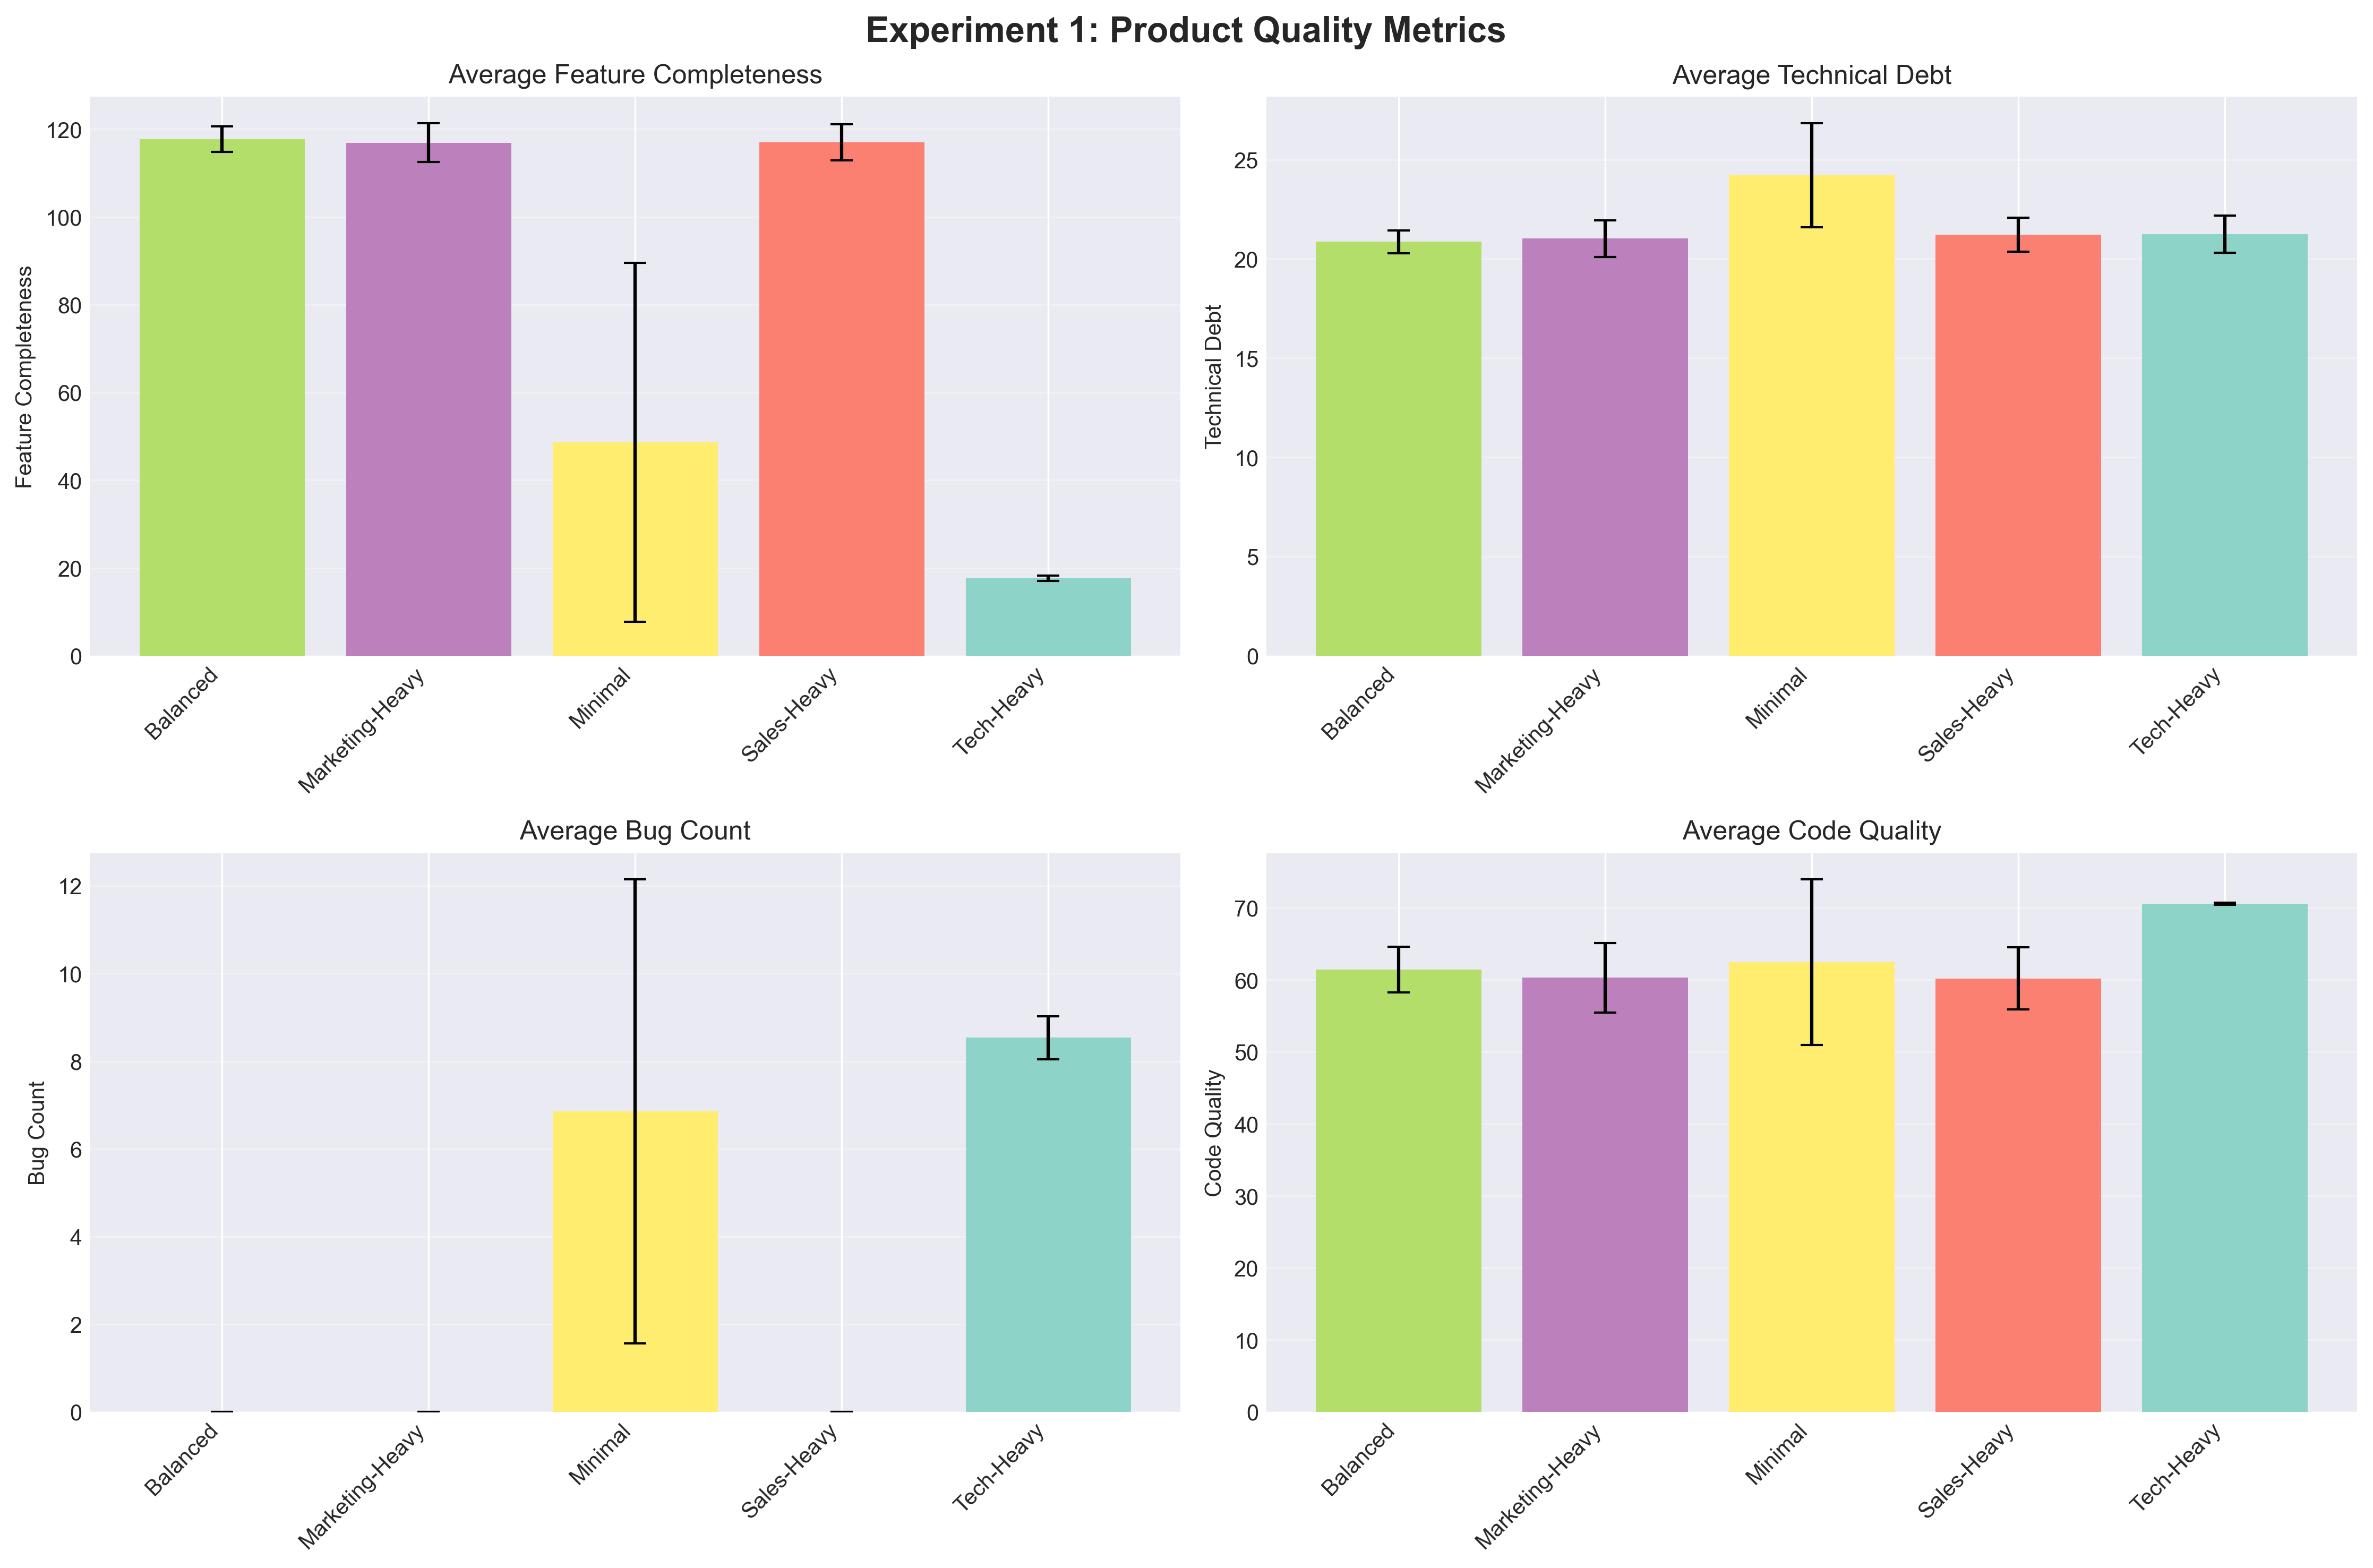
\includegraphics[width=\textwidth]{../results/exp3_product_quality_20260109_083536.png}
    \caption{Experiment 1: Product quality metrics reveal failure-driven degradation. Top-left: Features stratify. Top-right: Debt bifurcates. Bottom-left: Bugs separate failures from survivors. Bottom-right: Code quality clusters.}
    \label{fig:sup_exp3_quality}
\end{figure}

\begin{figure}[!htbp]
    \centering
    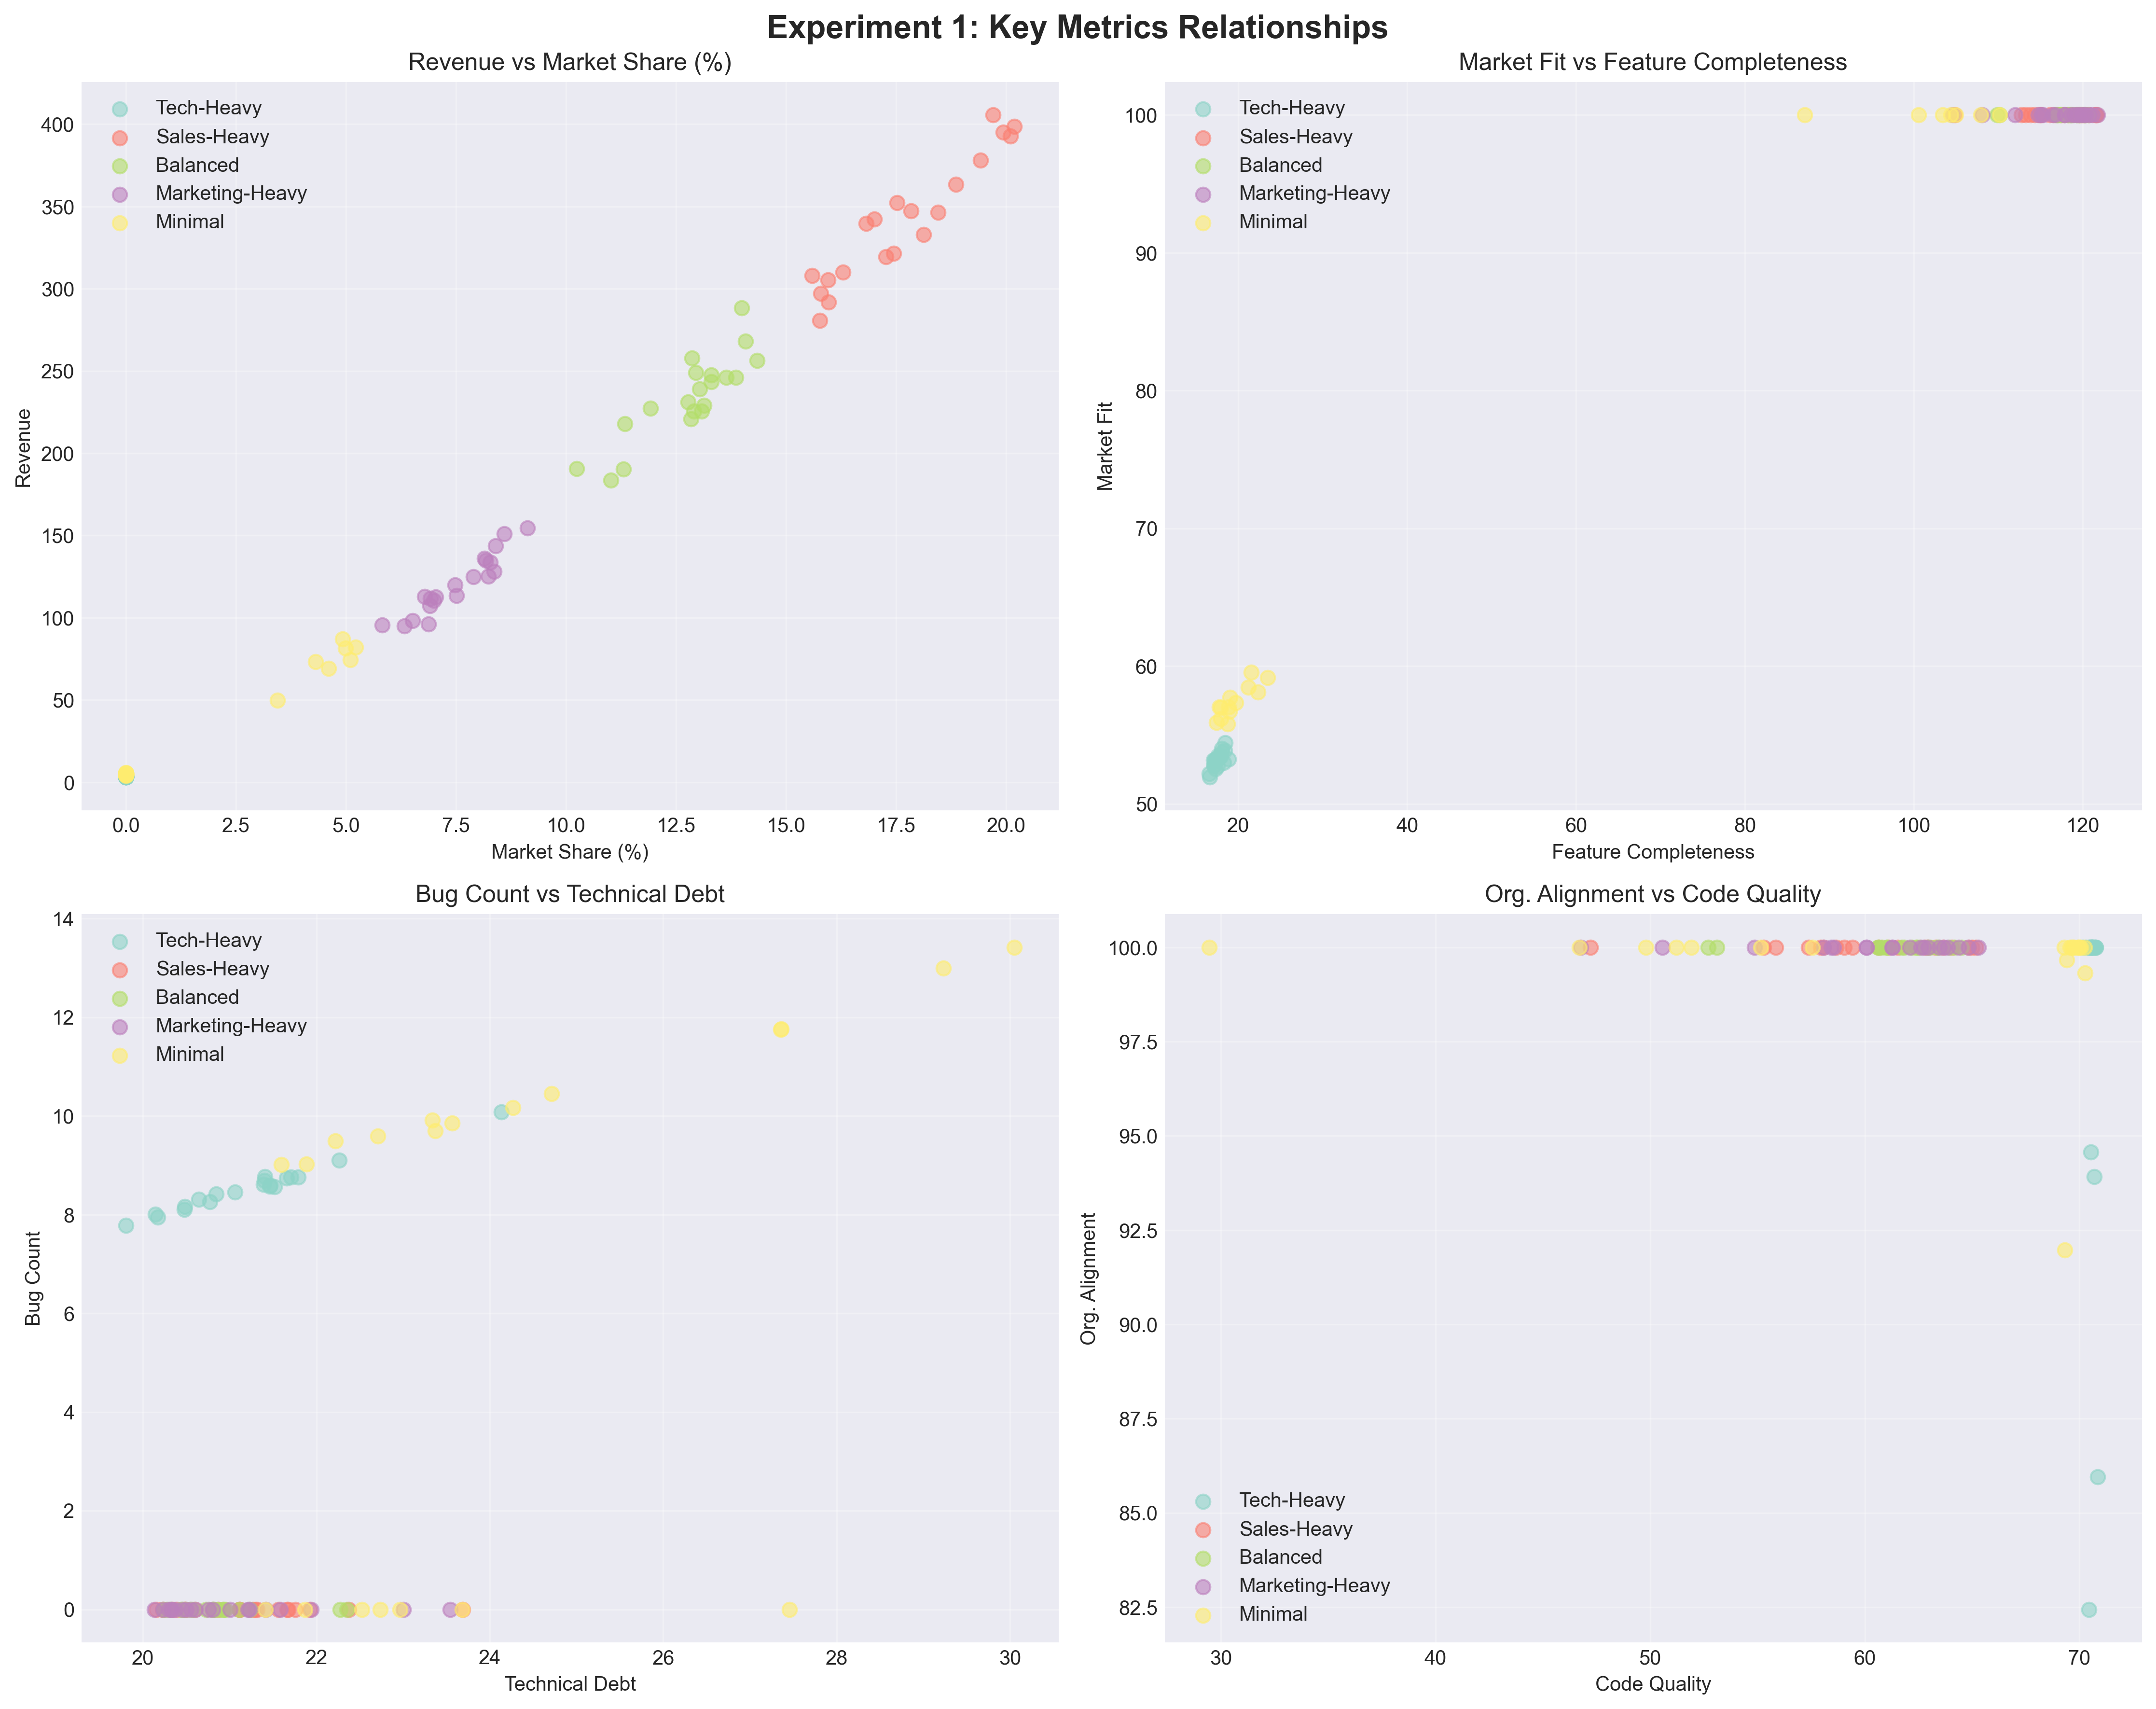
\includegraphics[width=\textwidth]{../results/exp3_relationships_20260109_083536.png}
    \caption{Experiment 1: Comparative metrics across configurations. Top-left: Revenue vs. market share. Top-right: Market fit reaches ceiling (100\%) for all survivors. Bottom-left: Technical debt and bugs remain zero for all survivors. Bottom-right: Organizational alignment.}
    \label{fig:sup_exp3_key_metrics}
\end{figure}

\begin{figure}[!htbp]
    \centering
    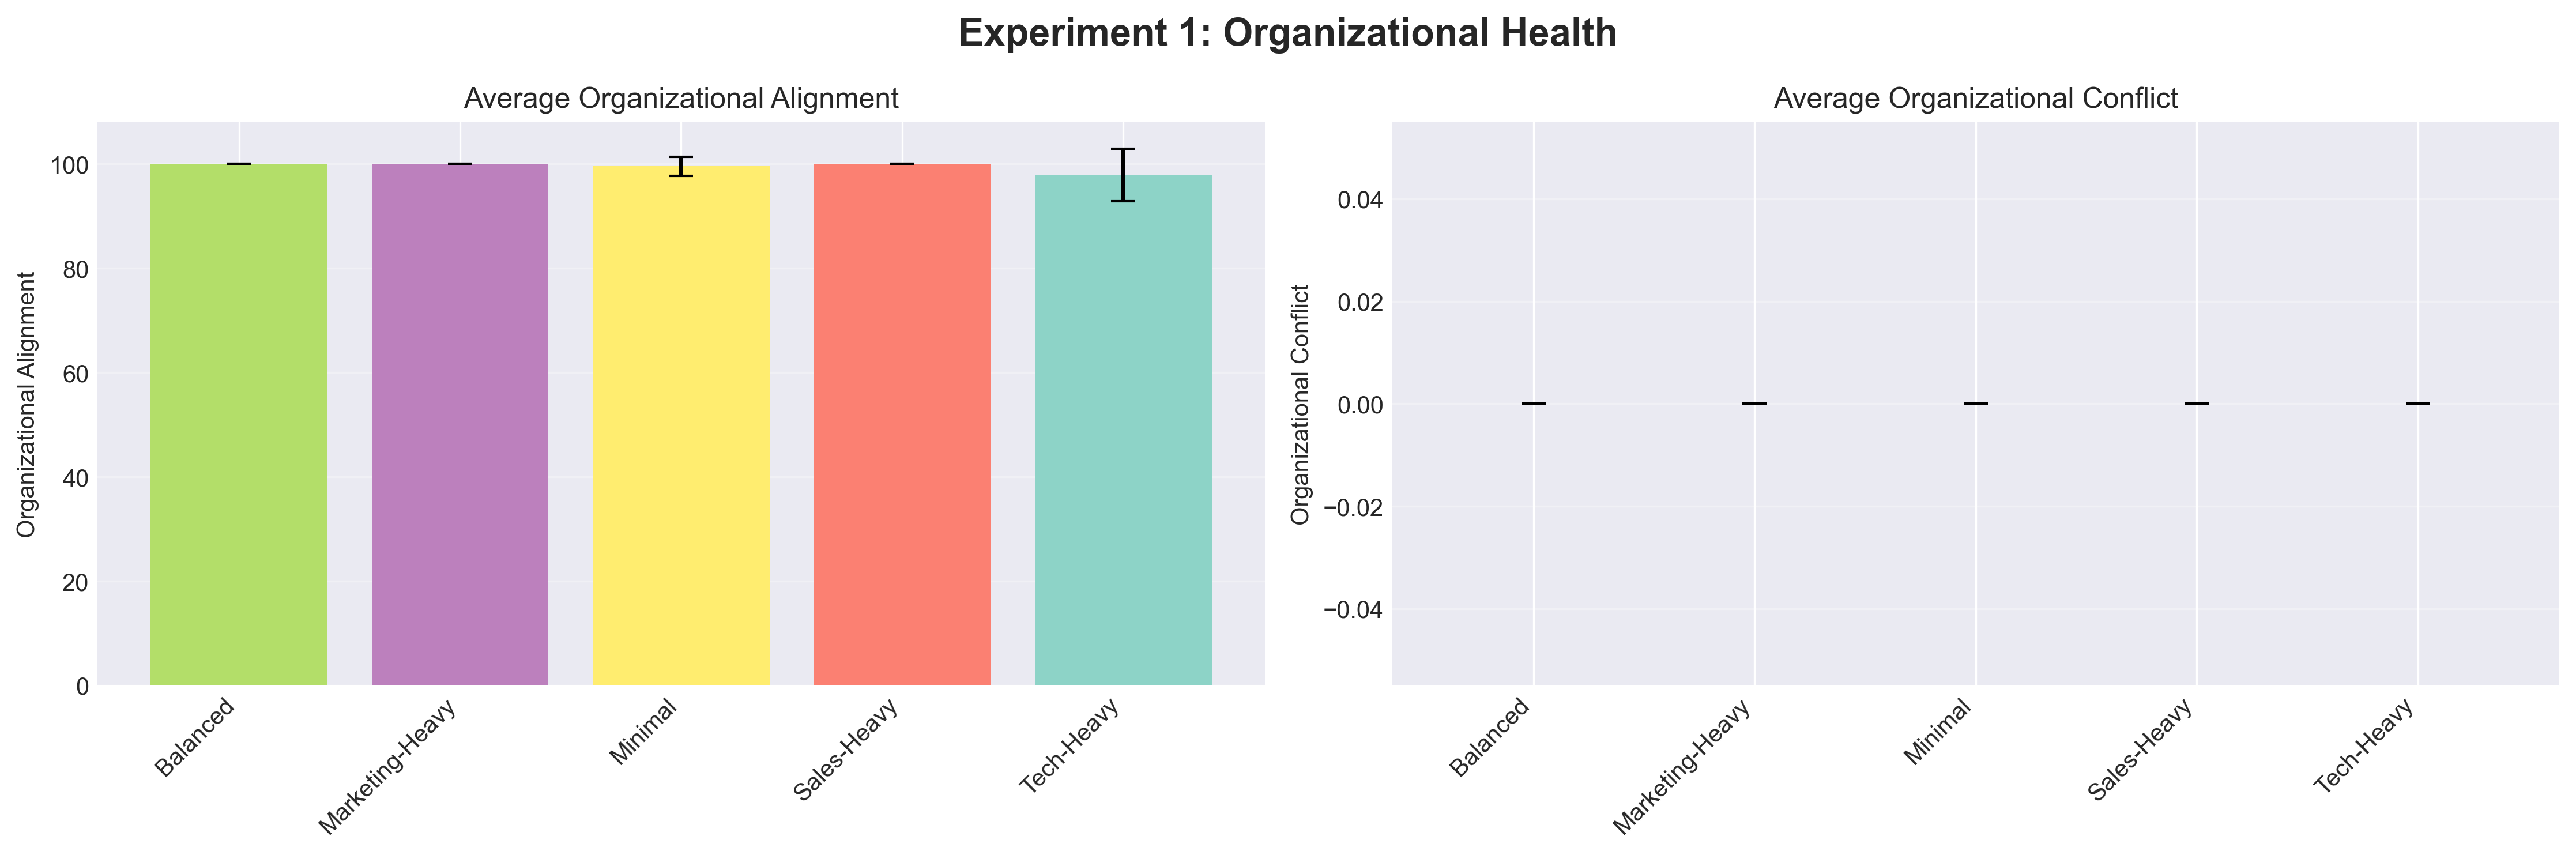
\includegraphics[width=\textwidth]{../results/exp3_organizational_20260109_083536.png}
    \caption{Experiment 1: Organizational health metrics show minimal differentiation. Left: Organizational alignment remains uniformly high. Right: Organizational conflict remains precisely zero for all configurations.}
    \label{fig:sup_exp3_org_health}
\end{figure}

\subsection{Experiment 2: Quality vs. Speed}

\begin{figure}[!htbp]
    \centering
    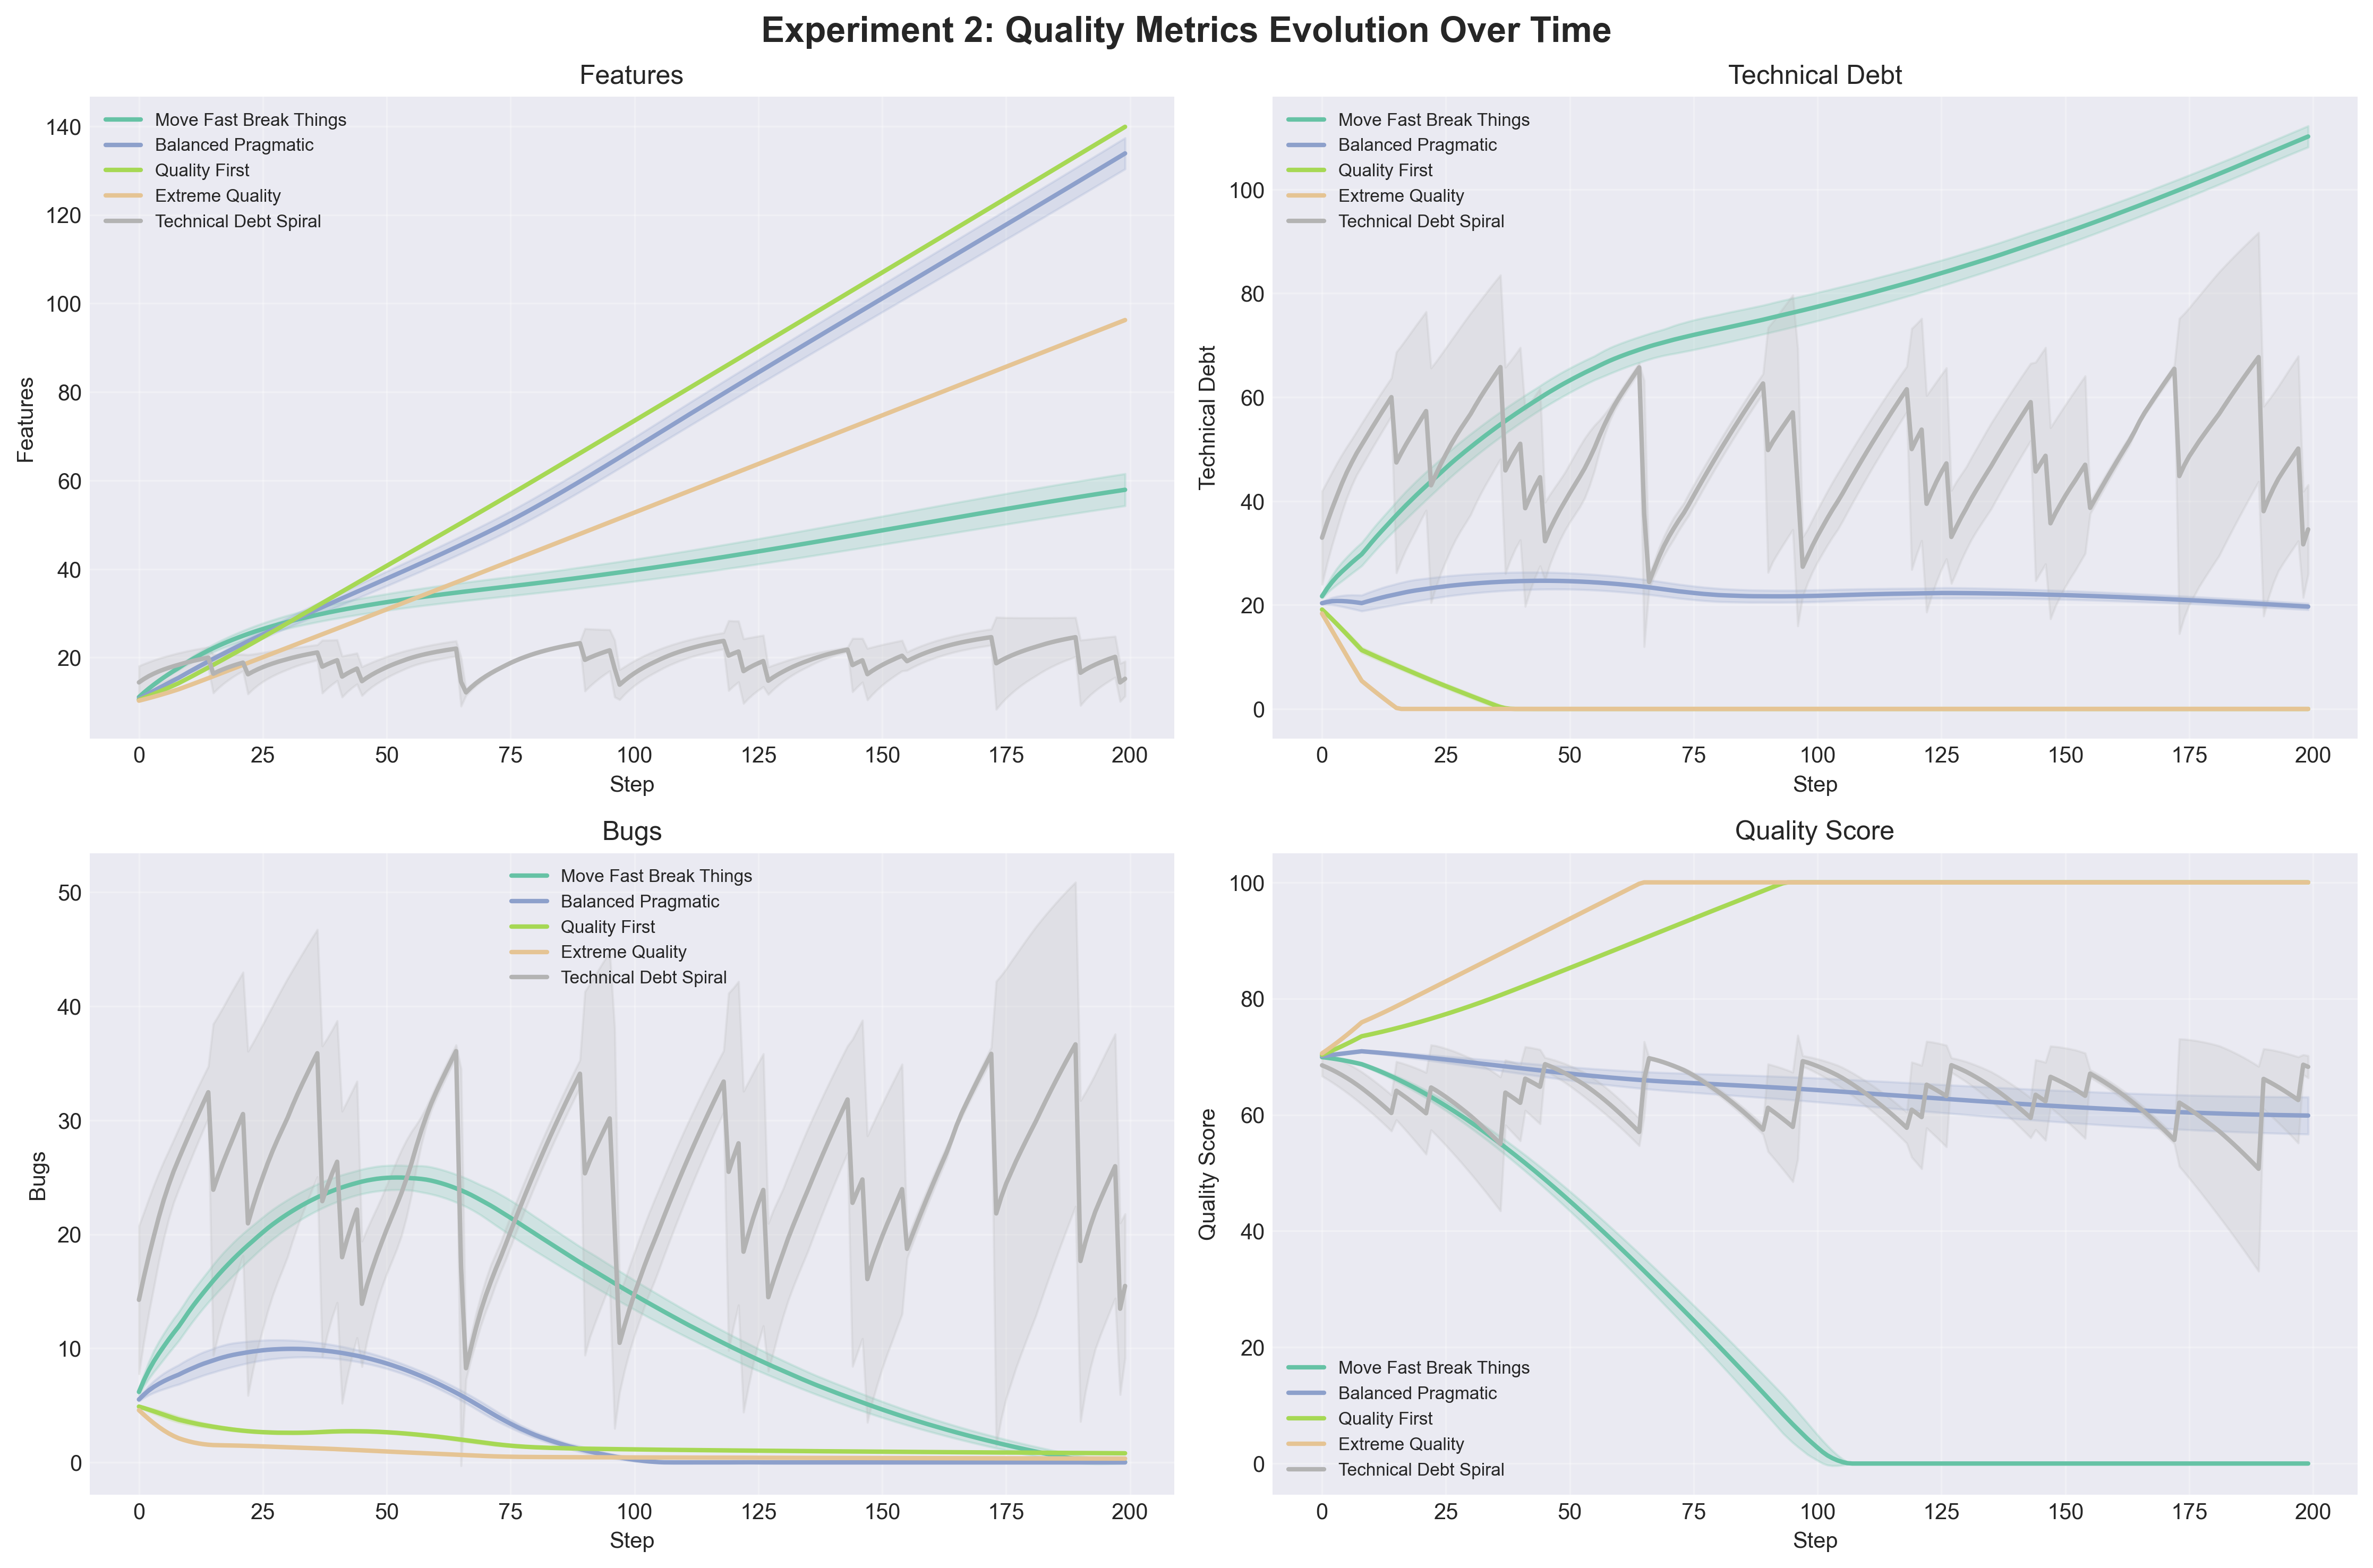
\includegraphics[width=\textwidth]{../results/exp4_quality_evolution_20260109_084356.png}
    \caption{Experiment 2: Quality metrics evolution demonstrates functional quality degradation mechanisms. Top-left: Features stratify by velocity. Top-right: Technical debt. Bottom-left: Bug count. Bottom-right: Code quality.}
    \label{fig:sup_exp2_quality_evolution}
\end{figure}

\begin{figure}[!htbp]
    \centering
    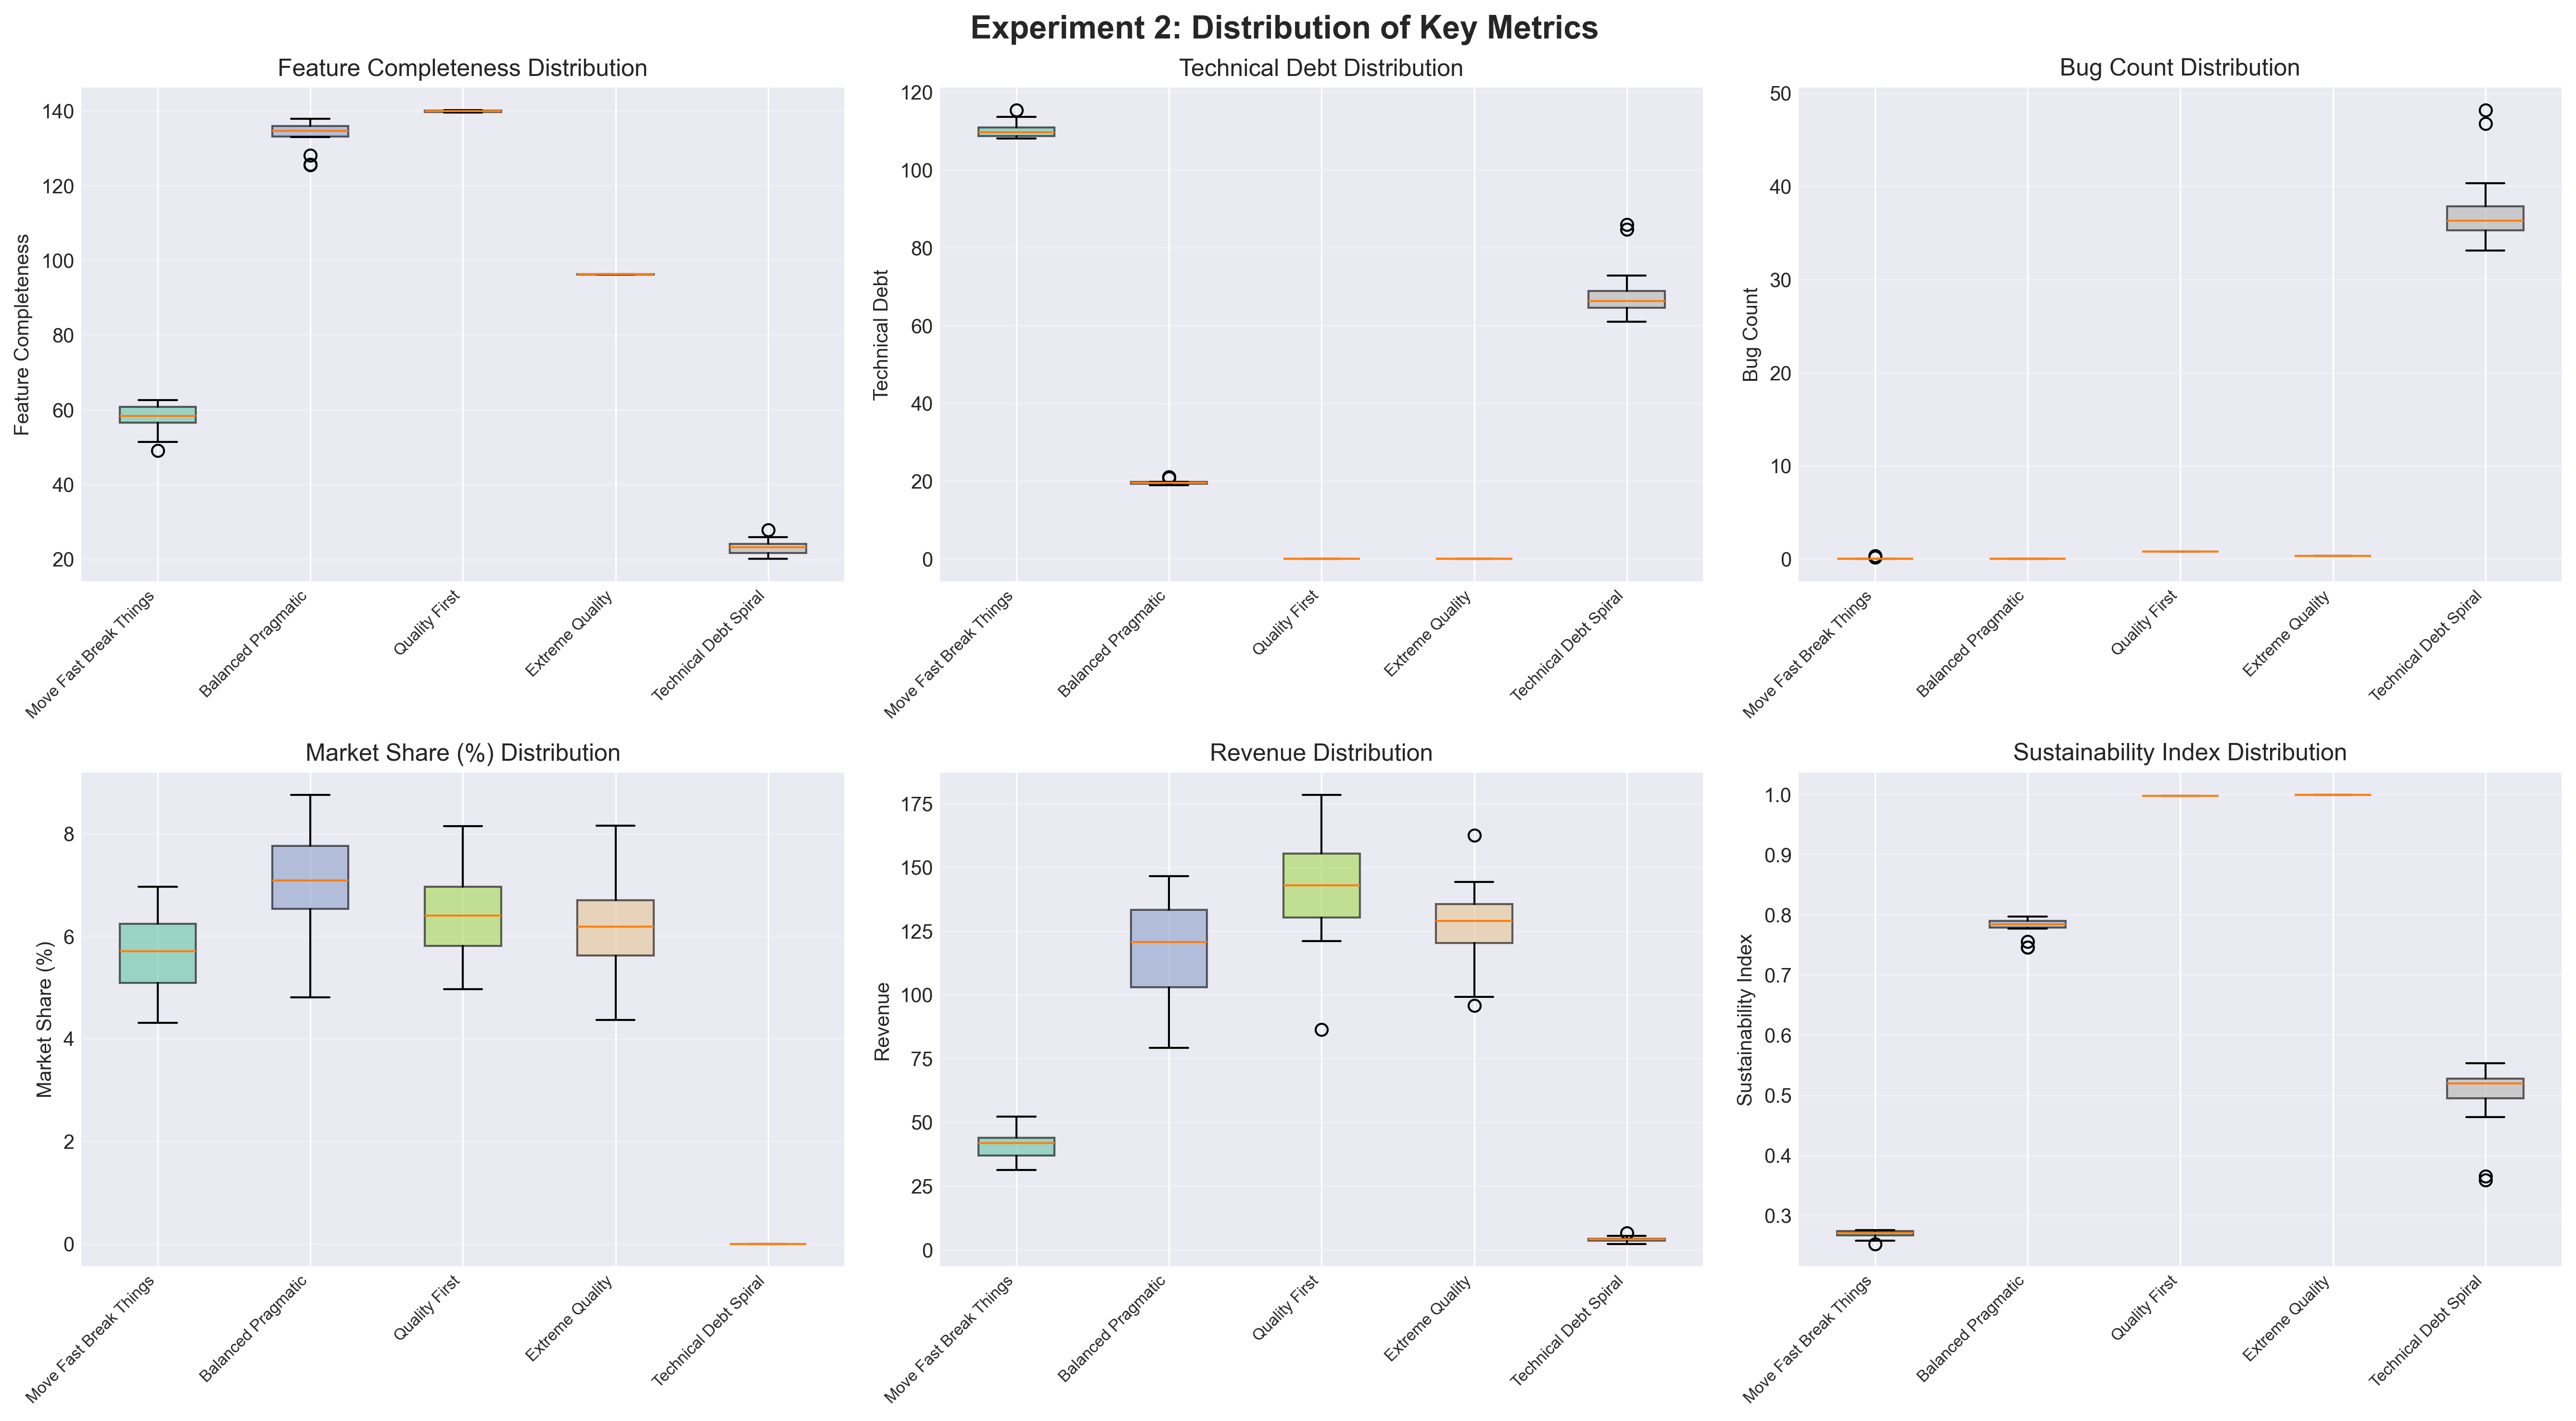
\includegraphics[width=\textwidth]{../results/exp4_distributions_20260109_084356.png}
    \caption{Experiment 2: Performance distributions reveal quality-velocity tradeoff emergence.}
    \label{fig:sup_exp2_distributions}
\end{figure}

\begin{figure}[!htbp]
    \centering
    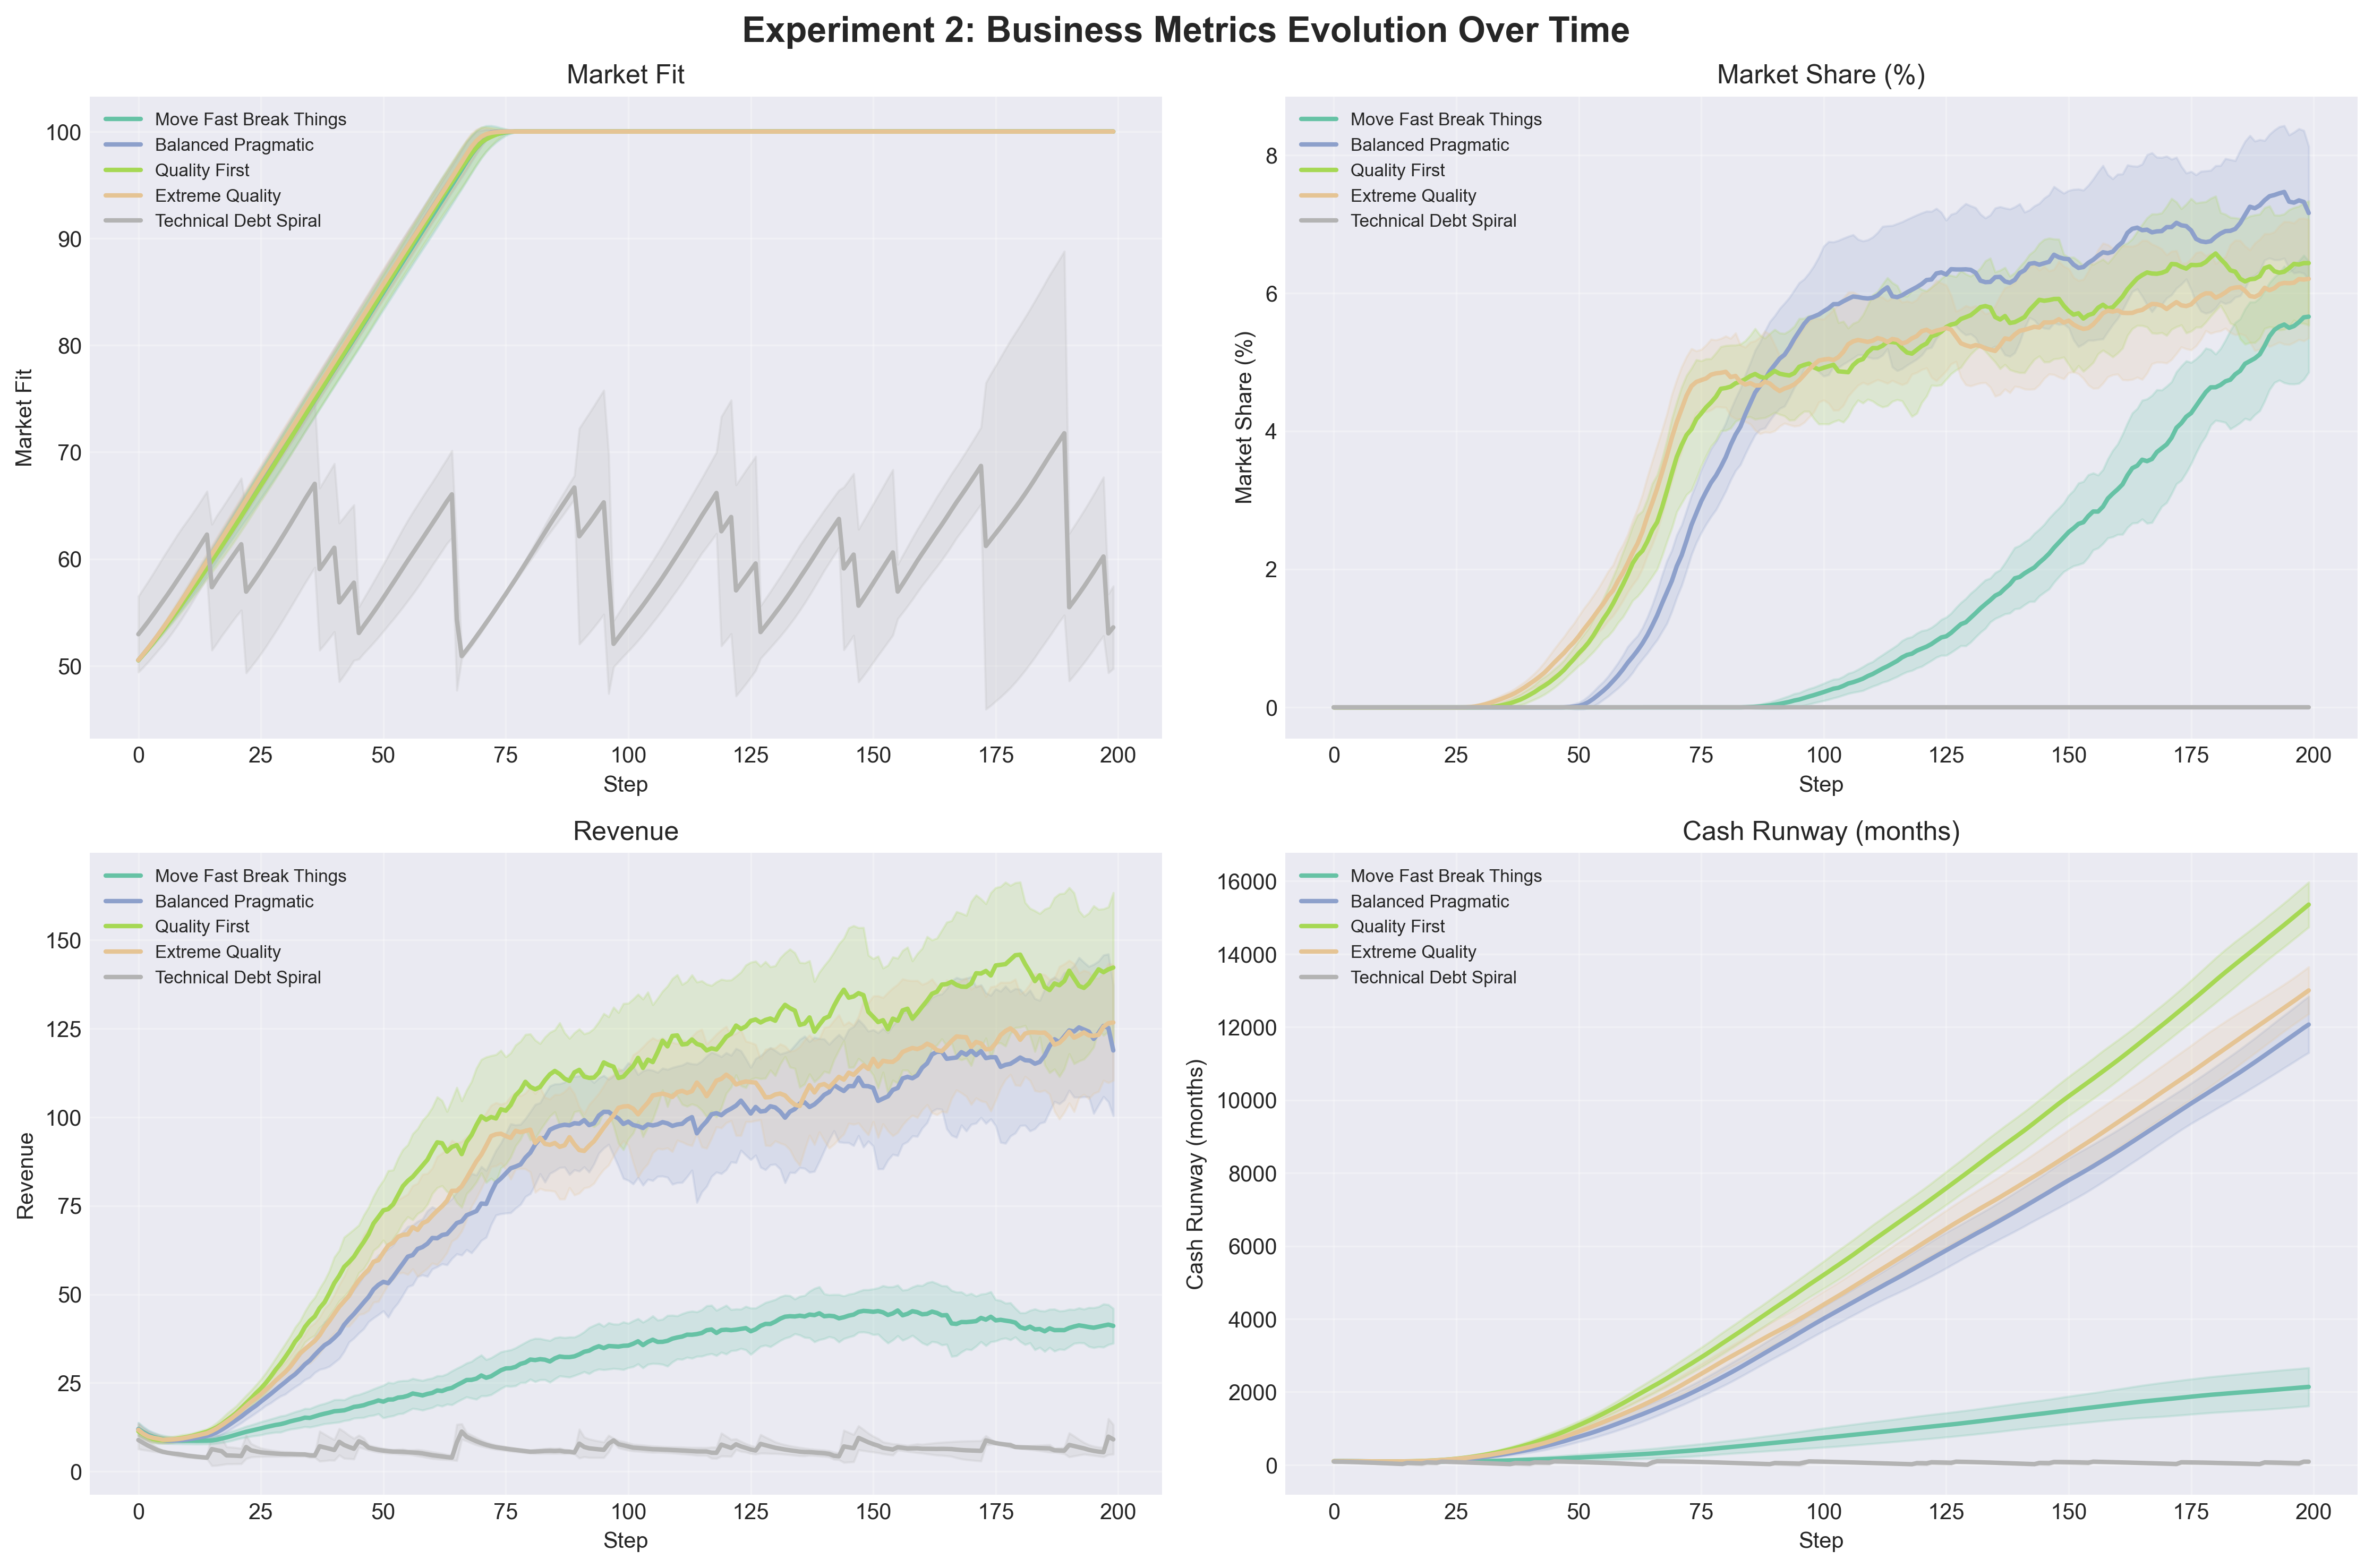
\includegraphics[width=\textwidth]{../results/exp4_business_evolution_20260109_084356.png}
    \caption{Experiment 2: Business metrics evolution shows quality-driven bifurcation.}
    \label{fig:sup_exp4_business}
\end{figure}

\subsection{Experiment 3: Initial Capital}

\begin{figure}[!htbp]
    \centering
    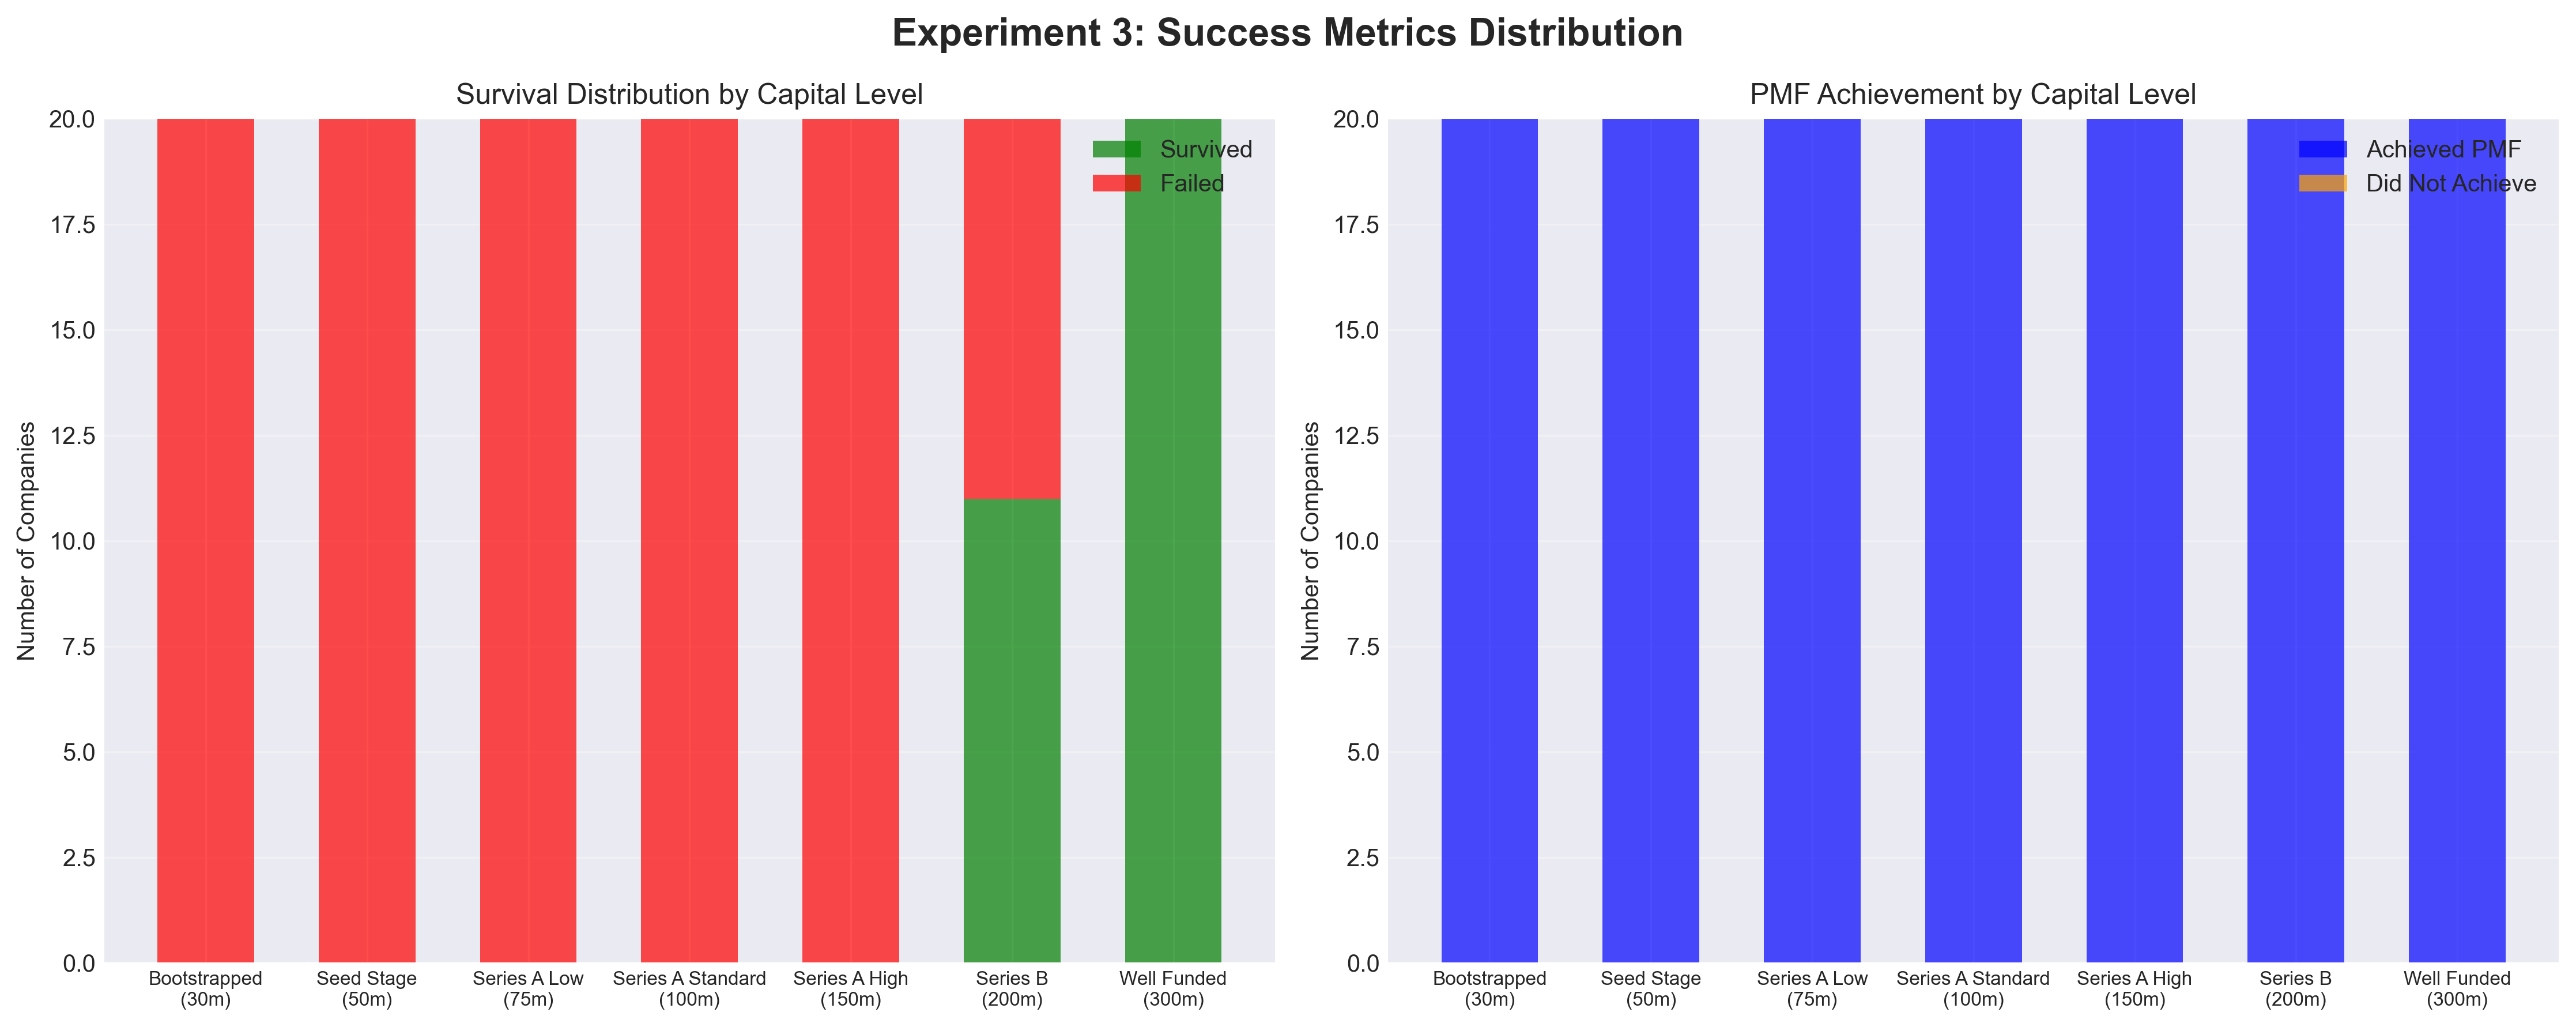
\includegraphics[width=\textwidth]{../results/exp5_distributions_20260109_101713.png}
    \caption{Experiment 3: Metric distributions by capital level.}
    \label{fig:sup_exp3_distributions}
\end{figure}

\begin{figure}[!htbp]
    \centering
    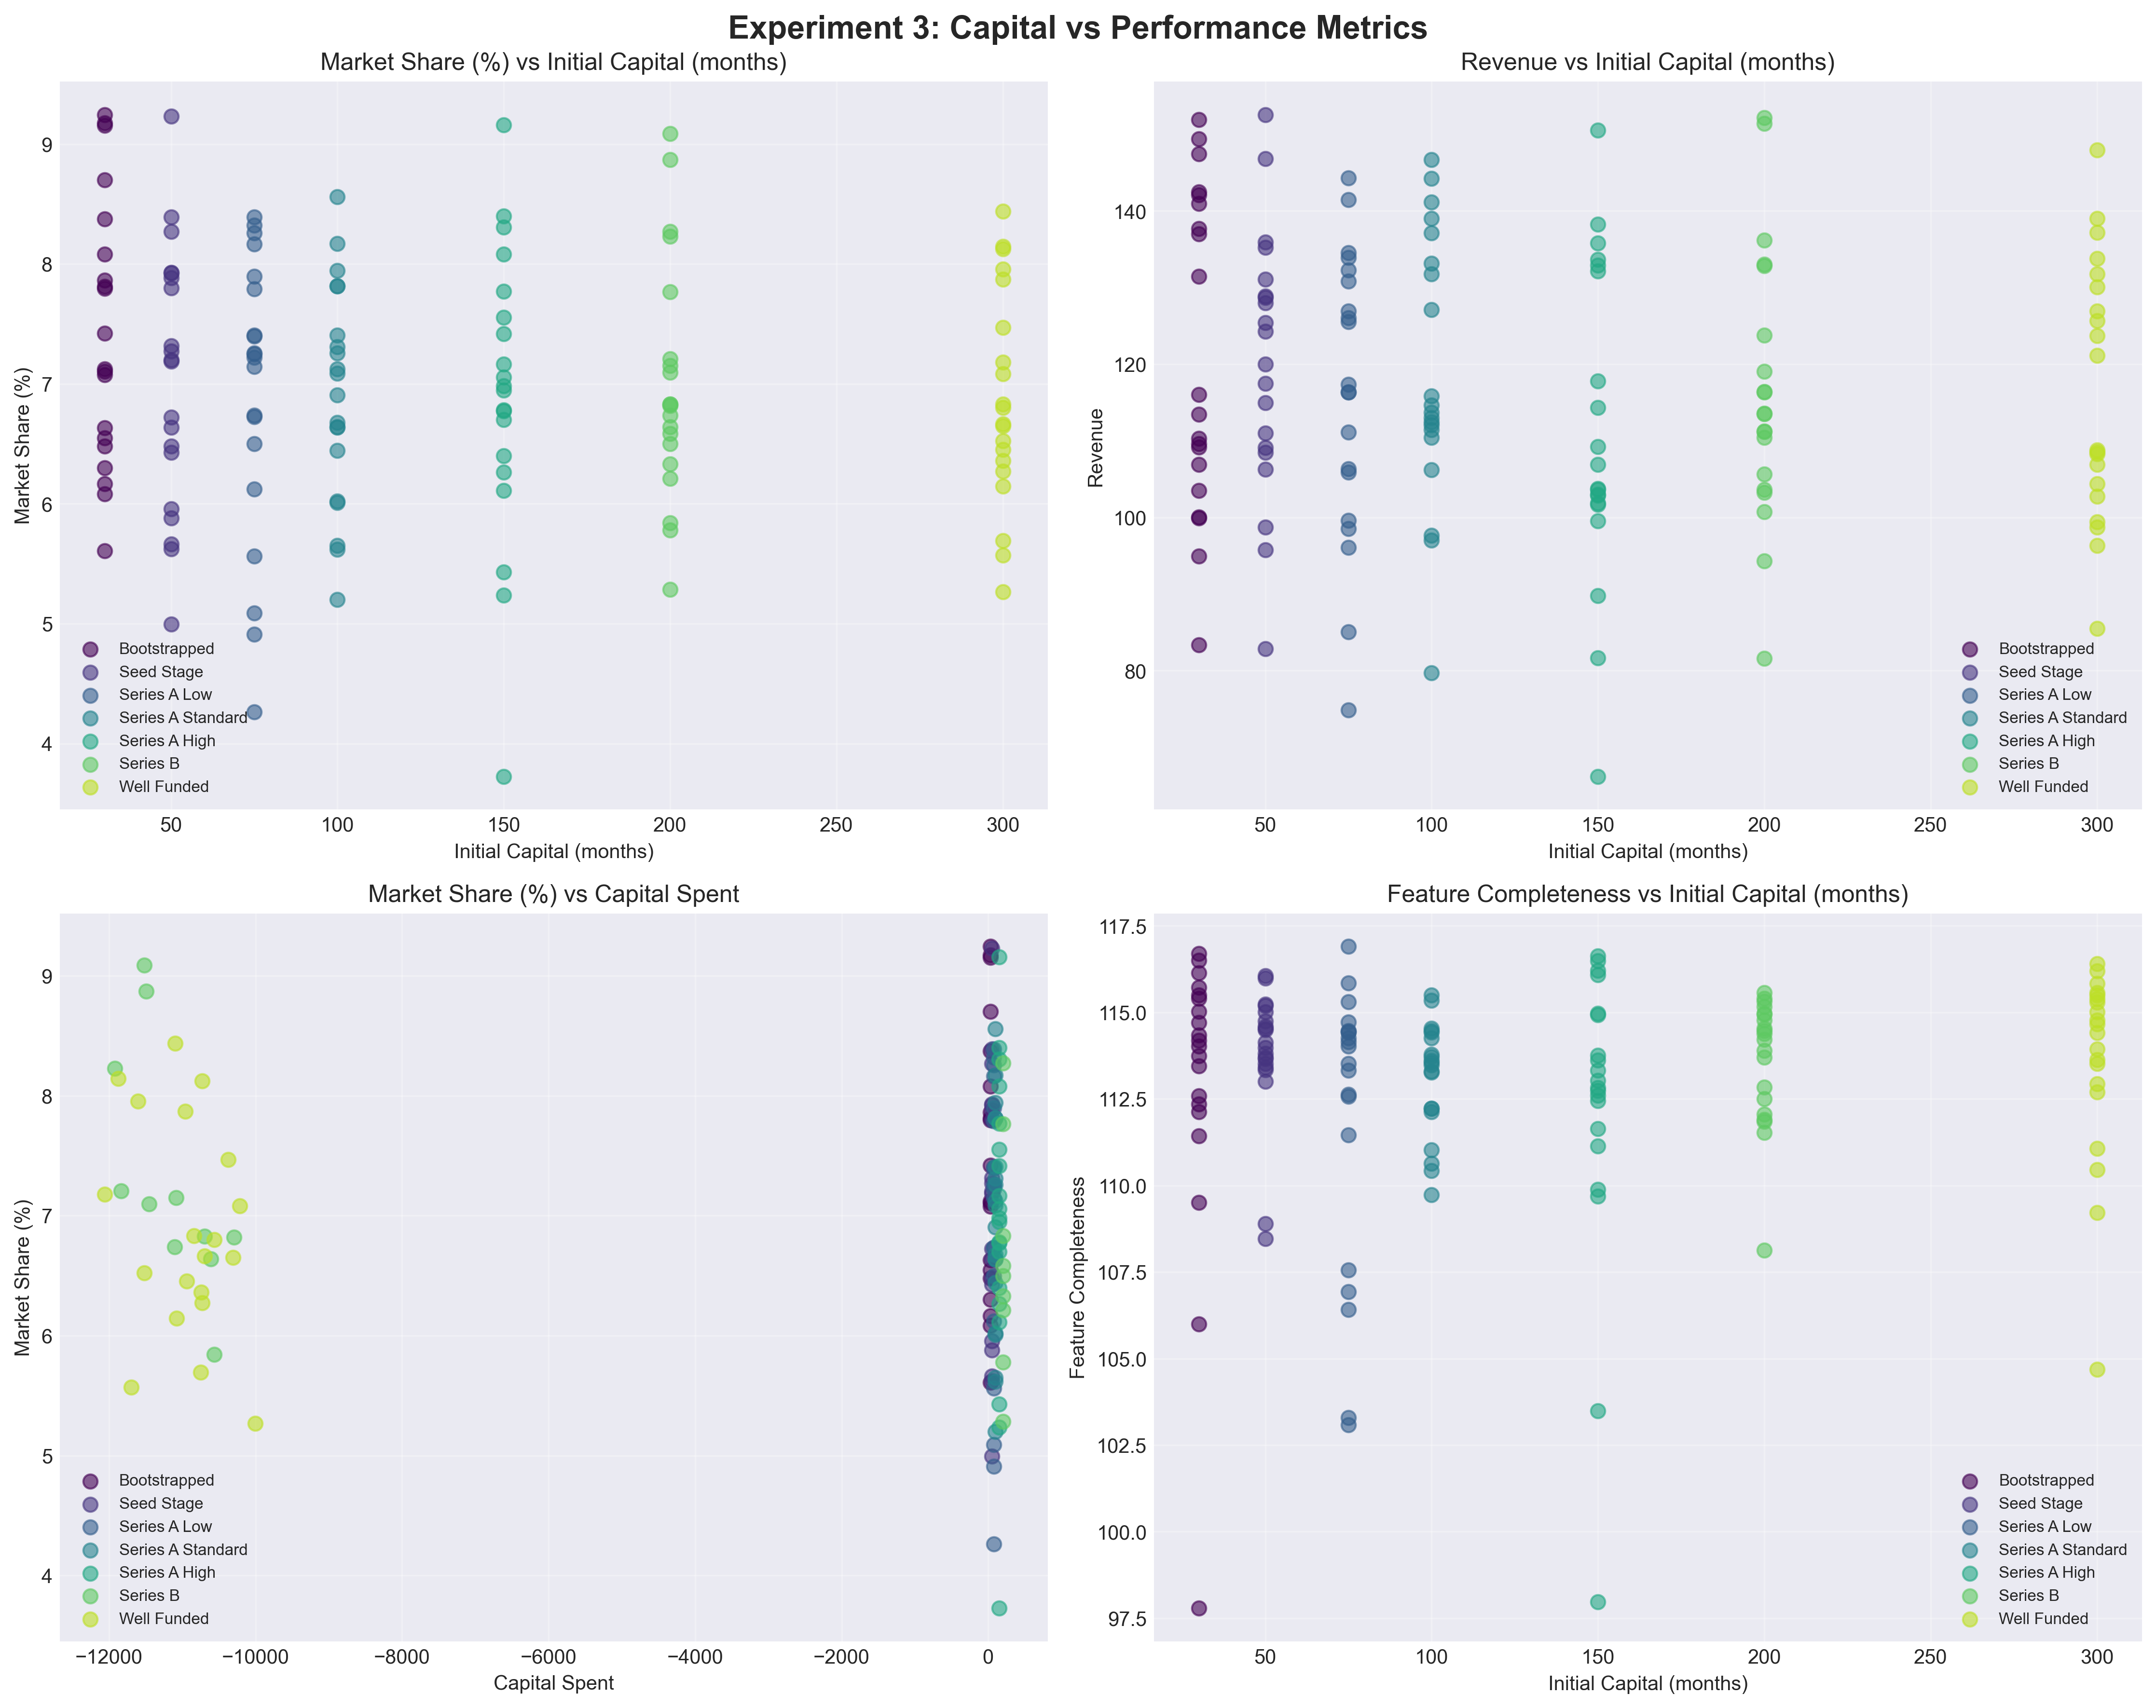
\includegraphics[width=\textwidth]{../results/exp5_scatter_20260109_101713.png}
    \caption{Experiment 3: Capital versus performance metrics.}
    \label{fig:sup_exp5_metrics}
\end{figure}

\selectlanguage{english}
\FloatBarrier

\end{document}
